\chapter{Degenerate and Compact Stars}
\label{ch:compact}

\newcommand{\ThirteenMchFormula}{1.456}
\newcommand{\ThirteenMwdLargest}{1.456}
\newcommand{\ThirteenRsiriusB}{5566}
\newcommand{\ThirteenMovMax}{0.71}
\newcommand{\ThirteenRovMax}{9.3}
\newcommand{\ThirteenMnsNewtonLargest}{5.69}
\newcommand{\ThirteenCompactOV}{0.11}


When a star has burned what it can, its core is left without a source of heat. It contracts, and by Section~\ref{sg:sec:negheat} it heats, until something other than heat holds it up. Two things can. The degeneracy pressure of electrons holds up white dwarfs, and that of neutrons holds up neutron stars. When neither suffices, nothing does, and the core becomes a black hole.

The word relativistic is used here in two separate senses, and keeping them apart is most of the chapter. Relativistic particles, electrons moving near the speed of light, soften the pressure to $\gamma=\tfrac43$, and that alone, in plain Newtonian gravity, sets the maximum mass of a white dwarf. Relativistic gravity changes the structure equations themselves, and it matters only when a star is compact enough. General relativity itself is not recapped. The relativistic forms below are quoted from it.

% ==============================================================================
\section{Compactness}
\label{cs:sec:compactness}

The equations of Chapter~\ref{ch:structure} used Newtonian gravity throughout.

They cannot hold for every star. A body compact enough must be described by general relativity, and the question is where the line falls.

Think of a ball thrown up from the surface of a small asteroid. A gentle throw sends it away for good. On the Earth the same throw brings it straight back. How hard gravity grips a body at the surface depends on how much mass is packed into how small a radius.

The grip of gravity, measured against the speed of light, is the ratio $GM/(Rc^2)$, the \textbf{compactness}. It compares the escape energy per unit mass at the surface with $c^2$. Every correction that general relativity makes to the structure of a star is of this size, so it decides whether Newtonian gravity is good enough (P6).

In numbers, the Sun has $GM/(Rc^2)=2.1\times10^{-6}$, the white dwarf Sirius B $2.6\times10^{-4}$, and a neutron star of $1.4\,M_\odot$ and $12\,\mathrm{km}$ radius $0.17$.

The picture is a scale running from $0$ to $\tfrac12$. The Sun sits at the bottom, white dwarfs a little above, neutron stars a third of the way up, and a black hole at the top.

The same ratio sets the gravitational redshift of light leaving a surface, the bending of starlight, and the share of rest mass released when matter falls onto a compact object. It gives the size of every relativistic correction.

\begin{table}[htbp]
	\centering
	\begin{tabular}{@{}l c c c@{}}
		\toprule
		\textbf{Object} & $GM/(Rc^2)$ & \textbf{surface redshift} $z$ & \textbf{gravity treated by} \\
		\midrule
		Sun & $2.1\times10^{-6}$ & $2.1\times10^{-6}$ & Newton \\
		Sirius B (white dwarf) & $2.6\times10^{-4}$ & $2.6\times10^{-4}$ & Newton \\
		Neutron star, $1.4\,M_\odot$, $12\,\mathrm{km}$ & $0.17$ & $0.24$ & general relativity \\
		Black hole & $0.5$ & -- & general relativity \\
		\bottomrule
	\end{tabular}
	\caption{Compactness and surface redshift, $z=(1-2GM/Rc^2)^{-1/2}-1$.}
	\label{cs:tab:compactness}
\end{table}

The redshift of Sirius B, $z=2.6\times10^{-4}$, shifts its spectral lines as a recession at $77\,\mathrm{km\,s^{-1}}$ would, close to what is measured. Why so dense a star can exist at all is worked out in Section~\ref{cs:sec:wd}, and Newtonian gravity is enough for it.

% ==============================================================================
\section{White Dwarfs}
\label{cs:sec:wd}

The pressure of degenerate electrons is a power of the density alone, $\rho^{5/3}$ for slow electrons and $\rho^{4/3}$ for fast ones (Eq.~\eqref{st:eq:degenerate_P}). A star held up by it is therefore a polytrope (Section~\ref{st:sec:polytropes}).

A white dwarf of the Sun's mass is the size of the Earth. As its mass grows, its electrons are squeezed harder and move faster. The polytrope of slow electrons cannot describe the heaviest ones.

Think of a crowd in a hall, pressed toward the front by a slope. Each person's push on the person behind grows the harder they are squeezed, at first. If everyone is already pushing as hard as they can, adding more people down the slope only crushes the front, and no new push appears to stop it.

Electrons near the speed of light behave like that crowd. Their momentum can keep growing, but their speed cannot exceed $c$, so their pressure grows more slowly with density, $\gamma\to\tfrac43$. By the virial theorem (Section~\ref{sg:sec:virial}), a star with $\gamma=\tfrac43$ is barely bound, and by the mass–radius relation \eqref{st:eq:mass_radius} only one mass fits. Above that mass, degenerate electrons cannot hold a star up. Counting states (P3) and the virial balance of a sphere (P1, P2) give that mass.

In numbers, the limit is $\ThirteenMchFormula\,M_\odot$ for the carbon and oxygen of white dwarfs, with two atomic mass units per electron, $\mu_e=2$.

The picture is Figure~\ref{cs:fig:wd}, the radius of white dwarfs shrinking as their mass grows, down to zero at the limit.

\begin{figure}[htbp]
	\centering
	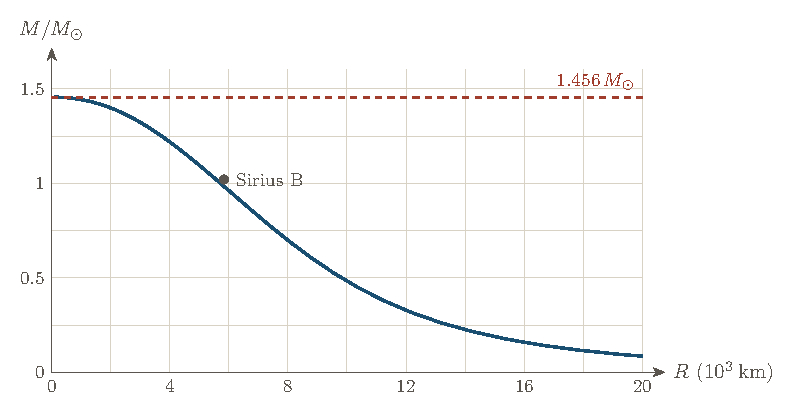
\includegraphics{fig_ch13_wd_mass_radius.pdf}
	\caption{The mass of white dwarfs against their radius, computed from the exact pressure of degenerate electrons with $\mu_e=2$. The dashed line marks $\ThirteenMchFormula\,M_\odot$. The dot marks the observed mass and radius of Sirius B.}
	\label{cs:fig:wd}
\end{figure}

The same limit sets the mass of the iron core of a massive star at the moment it collapses into a neutron star, and the mass at which a white dwarf gaining matter from a companion explodes as a type Ia supernova. It gives the mass–radius relation of white dwarfs and the Chandrasekhar mass, by two routes.

\paragraph{Slow electrons.} A light white dwarf has slow electrons, so $\gamma=\tfrac53$ and, by Eq.~\eqref{st:eq:mass_radius},
\begin{equation}
	R\propto M^{-1/3}.
\end{equation}
Adding mass makes it smaller. The degenerate pressure depends on the density alone, so a heavier star must be denser to hold itself up.

\paragraph{Fast electrons, the Chandrasekhar mass.} For fast electrons, $P=\mathcal K\rho^{4/3}$ with $\mathcal K=(hc/8)(3/\pi)^{1/3}/(\mu_em_{\rm u})^{4/3}$ from Eq.~\eqref{st:eq:degenerate_P} and $n_e=\rho/(\mu_em_{\rm u})$, where $m_{\rm u}$ is the atomic mass unit. With $\gamma=\tfrac43$, Eq.~\eqref{st:eq:r0} gives $r_0^2=\mathcal K\rho_c^{-2/3}/(\pi G)$, so $r_0^3\rho_c=(\mathcal K/\pi G)^{3/2}$ does not depend on $\rho_c$, and the mass formula of Section~\ref{st:sec:polytropes} gives one mass only,
\begin{align}
	M_{\rm Ch}
	&\eqby{1} 4\pi\Big[-\xi^2\dv{\theta}{\xi}\Big]_{\xi_1}\left(\frac{\mathcal K}{\pi G}\right)^{3/2} \nonumber\\
	&\eqby{2} 4\pi\times\TwelveOmegaThree\times\left(\frac{hc}{8\pi G}\right)^{3/2}\left(\frac3\pi\right)^{1/2}\frac{1}{(\mu_em_{\rm u})^2} .
\end{align}
\begin{explain}
	\item The mass of a polytrope, $4\pi r_0^3\rho_c[-\xi^2\theta']_{\xi_1}$, with $r_0^3\rho_c=(\mathcal K/\pi G)^{3/2}$.
	\item The Lane–Emden value for $\gamma=\tfrac43$ and $\mathcal K$ written out.
\end{explain}
\begin{equation}
	\boxed{M_{\rm Ch}=\frac{5.83}{\mu_e^2}\,M_\odot=\ThirteenMchFormula\,M_\odot\quad(\mu_e=2).}
	\label{cs:eq:chandrasekhar}
\end{equation}
The mass contains $h$, $c$, $G$ and the mass per electron, and nothing about the star's history. Quantum mechanics ($h$), relativity ($c$) and gravity ($G$) together fix a mass of the order of the Sun's.

\paragraph{The same mass by an energy argument.} Landau found the limit by comparing two energies of one electron in a star of $N$ electrons and radius $R$. Its share of gravitational energy is about $-GM\mu_em_{\rm u}/R$, with $M=N\mu_em_{\rm u}$. A fast electron confined to a spacing $R/N^{1/3}$ has, by the uncertainty principle, a momentum of about $\hbar N^{1/3}/R$ and so a kinetic energy of about $\hbar cN^{1/3}/R$. Both scale as $1/R$, so shrinking the star changes their ratio not at all (P6). If gravity wins at one radius, it wins at every radius, and the star collapses. The two are equal when
\begin{align}
	\frac{\hbar c\,N^{1/3}}{R}
	&= \frac{G\,N(\mu_em_{\rm u})^2}{R} \nonumber\\
	\implies\quad N
	&= \left(\frac{\hbar c}{G(\mu_em_{\rm u})^2}\right)^{3/2},\qquad
	M=N\mu_em_{\rm u}=\left(\frac{\hbar c}{G}\right)^{3/2}\frac{1}{(\mu_em_{\rm u})^2}.
\end{align}
This is $0.47\,M_\odot$ for $\mu_e=2$. The estimate has the right combination of constants and falls short of Eq.~\eqref{cs:eq:chandrasekhar} only by a number, $3.1$, that the full polytrope supplies.

\paragraph{The full curve.} Real white dwarfs have electrons that are neither slow nor at the speed of light. Figure~\ref{cs:fig:wd} uses the exact pressure of degenerate electrons at any speed, integrated in Newtonian hydrostatic equilibrium. Light white dwarfs follow $R\propto M^{-1/3}$. As the mass rises toward $\ThirteenMchFormula\,M_\odot$ the radius falls to zero. Sirius B, $1.02\,M_\odot$, lies on the curve at $\ThirteenRsiriusB\,\mathrm{km}$, against $5840\,\mathrm{km}$ measured, close enough given that the model ignores temperature and composition details. Throughout, $GM/(Rc^2)<10^{-3}$, so Newtonian gravity is enough. The limit comes from the particles being relativistic, not gravity.

% ==============================================================================
\section{The Relativistic Structure Equations}
\label{cs:sec:relativistic}

The four structure equations of Section~\ref{st:sec:four_equations} assumed Newtonian gravity.

A neutron star has $GM/(Rc^2)\approx0.2$. Corrections of that size cannot be dropped, and each equation must be replaced by its general-relativistic form.

Think of weighing a box of hot gas. Heat the gas and the box gets heavier, because energy has mass. Squeeze the gas and its pressure adds to the weight as well. In everyday life the extra weight is far too small to notice.

In a neutron star it is not small. The pressure that holds the star up is itself a source of gravity, so pushing harder also pulls harder. General relativity, with conservation of energy and momentum (P1) in curved space-time, gives the equations. They are quoted here from general relativity, not derived again.

In numbers, the pressure at the centre of a neutron star is between about a tenth and a half of its energy density $\rho c^2$. At the centre of the Sun the same ratio is about $2\times10^{-6}$.

The picture is the Newtonian structure equations of Section~\ref{st:sec:four_equations}, each with a few correction factors, every one of them close to one when $GM/(rc^2)$ and $P/(\rho c^2)$ are small.

The same equations, in the form given by Thorne (1977), are used for neutron stars, for the hottest proto-neutron stars just after a supernova, and for any star compact enough. They give the full relativistic set, side by side with the Newtonian one.

\paragraph{The metric.} A static spherical star has the metric
\begin{equation}
	ds^2=-e^{2\Phi/c^2}c^2dt^2+\left(1-\frac{2Gm(r)}{rc^2}\right)^{-1}dr^2+r^2\big(d\theta^2+\sin^2\theta\,d\phi^2\big),
\end{equation}
where $\Phi(r)$ becomes the Newtonian potential of Section~\ref{pr:sec:p2} far from the star, and $m(r)$ is the mass inside $r$.

\begin{table}[htbp]
	\centering
	\renewcommand{\arraystretch}{2.0}
	\begin{tabular}{@{}l l l@{}}
		\toprule
		& \textbf{Newtonian} & \textbf{General relativity} \\
		\midrule
		Mass & $\dv{m}{r}=4\pi r^2\rho$ & $\dv{m}{r}=4\pi r^2\rho$, \ $\rho c^2=$ total energy density \\
		Momentum & $\dv{P}{r}=-\dfrac{Gm\rho}{r^2}$ & $\dv{P}{r}=-\dfrac{G\big(\rho+\frac{P}{c^2}\big)\big(m+\frac{4\pi r^3P}{c^2}\big)}{r^2\big(1-\frac{2Gm}{rc^2}\big)}$ \\
		Potential & $\dv{\Phi}{r}=\dfrac{Gm}{r^2}$ & $\dv{\Phi}{r}=-\dfrac{c^2}{\rho c^2+P}\,\dv{P}{r}$ \\
		Energy & $\dv{L}{r}=4\pi r^2\rho\,\varepsilon$ & $\dv{r}\Big(L\,e^{2\Phi/c^2}\Big)=\dfrac{4\pi r^2\rho\,\varepsilon\,e^{2\Phi/c^2}}{\sqrt{1-2Gm/rc^2}}$ \\
		Transport & $L=-\dfrac{16\pi ac\,r^2T^3}{3\kappa\rho}\,\dv{T}{r}$ & $L=-\dfrac{16\pi ac\,r^2T^3}{3\kappa\rho}\,\sqrt{1-\tfrac{2Gm}{rc^2}}\;e^{-\Phi/c^2}\,\dv{r}\Big(T\,e^{\Phi/c^2}\Big)$ \\
		\bottomrule
	\end{tabular}
	\caption{The structure equations of a static star in Newtonian gravity and in general relativity (energy equation in a star that does not change).}
	\label{cs:tab:relativistic}
\end{table}

\paragraph{Reading the corrections.} The momentum equation is the Tolman–Oppenheimer–Volkoff (TOV) equation. Each of its three new factors is one physical effect.
\begin{itemize}
	\item $\rho+P/c^2$ in place of $\rho$. Pressure has inertia. A parcel under pressure is harder to hold up.
	\item $m+4\pi r^3P/c^2$ in place of $m$. Pressure gravitates. The pressure that holds the star up adds to the pull it must resist.
	\item $(1-2Gm/rc^2)^{-1}$. Space inside the star is curved, and the radial distance is longer than $dr$.
\end{itemize}
All three make gravity stronger. Raising the pressure to support more mass also raises gravity, so beyond some mass no equation of state can win. This is why neutron stars, unlike white dwarfs, have a maximum mass set by gravity itself, whatever the particles.

The energy equation conserves the luminosity as seen from far away, $L\,e^{2\Phi/c^2}$, where one factor $e^{\Phi/c^2}$ is the redshift of each photon's energy and the other is the slowing of clocks deep in the potential. The square root turns $dr$ into a proper volume.

\paragraph{Equilibrium in a gravitational field.} With no heat flow, $L=0$, the transport equation gives not a uniform $T$ but
\begin{equation}
	\boxed{T\,e^{\Phi/c^2}=\text{constant}.}
	\label{cs:eq:tolman}
\end{equation}
This is the Tolman–Ehrenfest relation. In a gravitational field, a body in full thermal equilibrium is hotter at the bottom, by the same factor by which light climbing out is redshifted. Heat flows only when $T\,e^{\Phi/c^2}$ changes from place to place. The statement in Section~\ref{sg:sec:rotation} that global equilibrium means one temperature throughout is the Newtonian limit of this. For the Sun the difference is two parts in a million. Across a neutron star it is about twenty percent.

\paragraph{Mass and binding.} In general relativity $m(r)$ counts the total energy inside $r$, including the negative gravitational binding energy. The mass $M$ that governs an orbit around the star is smaller than the rest mass of all its particles, by about $GM/(Rc^2)$ of it. For a neutron star the difference is about a tenth of the rest mass, $3\times10^{46}\,\mathrm J$, released when the core collapses, almost all of it as neutrinos (Problem~\ref{cs:prob:binding}).

% ==============================================================================
\section{Computing a Neutron Star}
\label{cs:sec:ns}

Table~\ref{cs:tab:relativistic} gives the equations, and the core of a collapsed star gives the material, neutrons packed to nuclear density.

How are the mass and radius of a neutron star actually found, and what does general relativity do to them?

Think of stacking sand into a cone. Pour more and the cone grows wider and taller. With dry sand the slope holds, and the cone can grow as large as the sand allows. With wet sand the weight of the top crushes the bottom past some height. Then the pile only spreads, and adding sand does not make it taller.

A neutron star is built in the same spirit, one central density at a time. Each central density gives one star, with its own mass and radius. Going to higher central density gives heavier stars, up to a point beyond which the extra gravity of the extra pressure wins and the mass falls. That point is the maximum mass. Finding it is the TOV equation (P1 and P2 in general relativity) solved with the pressure of degenerate neutrons (P3).

In numbers, an ideal gas of neutrons in general relativity reaches at most $\ThirteenMovMax\,M_\odot$, at a radius of $\ThirteenRovMax\,\mathrm{km}$. The same gas in Newtonian gravity reaches about $\ThirteenMnsNewtonLargest\,M_\odot$, eight times more.

The picture is Figure~\ref{cs:fig:ns}, two mass–radius curves for the same neutron gas, one turning over at a small mass.

\begin{figure}[htbp]
	\centering
	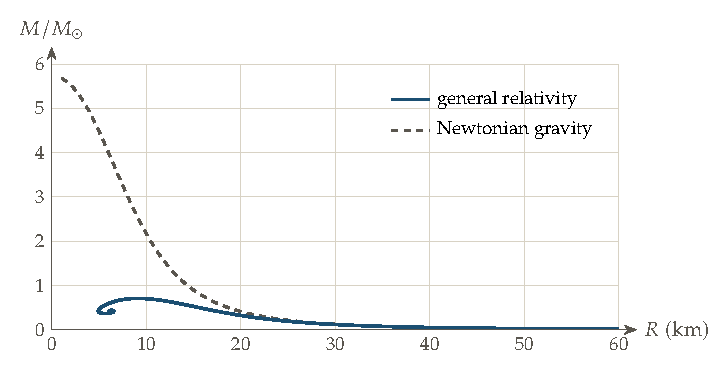
\includegraphics{fig_ch13_ns_mass_radius.pdf}
	\caption{Mass against radius for stars of an ideal degenerate neutron gas, computed with the TOV equation (solid) and with Newtonian hydrostatic equilibrium (dashed). Each point is one central density.}
	\label{cs:fig:ns}
\end{figure}

The same procedure, with the best equations of state from nuclear physics, gives the mass–radius curves that are tested against measured neutron-star masses and radii. It gives the procedure and what it shows.

\paragraph{The procedure.} A cold neutron star has no burning and no heat flow that matter for its structure, so only the mass and momentum equations of Table~\ref{cs:tab:relativistic} are needed, with an equation of state $P(\rho)$.
\begin{enumerate}
	\item Choose a central density $\rho_c$, so $P(0)=P(\rho_c)$ and $m(0)=0$.
	\item Integrate $\dv*{m}{r}$ and the TOV equation outward until $P=0$. That radius is $R$ and $m(R)$ is $M$.
	\item Repeat for a range of $\rho_c$. Each gives one point $(R,M)$.
\end{enumerate}
Both boundary conditions sit at the centre, unlike the two-ended problem of Section~\ref{st:sec:computing}, so a single outward integration finishes each star. Along the curve, stars with $\dv*{M}{\rho_c}>0$ are stable. Past the maximum, where $\dv*{M}{\rho_c}<0$, a small squeeze grows instead of rebounding.

\paragraph{What the curves show.} Figure~\ref{cs:fig:ns} uses the exact pressure of an ideal degenerate neutron gas, and its total energy density as the source of gravity. At low mass, where the star is large and $GM/(Rc^2)$ small, the two curves agree. As the mass grows they part. The Newtonian curve climbs toward the Chandrasekhar-like limit for neutrons, about $5.7\,M_\odot$, the $\mu_e=1$ value of Eq.~\eqref{cs:eq:chandrasekhar}. The relativistic curve turns over at $\ThirteenMovMax\,M_\odot$, the Oppenheimer–Volkoff limit, where $GM/(Rc^2)=\ThirteenCompactOV$. General relativity has cut the maximum mass by a factor of eight. Pressure that gravitates defeats itself.

\paragraph{Real neutron stars.} Pulsars in binaries are weighed with the timing methods of Chapter~\ref{ch:twobody} (Section~\ref{sec:romer}), and some are found at about $2\,M_\odot$, far above $\ThirteenMovMax\,M_\odot$. Neutrons are not an ideal gas. Nuclear forces repel them strongly at the highest densities and stiffen the pressure, and the best equations of state give maximum masses of about $2$ to $2.3\,M_\odot$. The maximum mass itself, and its derivation in general relativity, are taken here from the theory of compact objects, not derived again.

% ==============================================================================
\section{Black Holes}
\label{cs:sec:bh}

Above the maximum mass of a neutron star, no pressure can stop a collapse. By the reading of the TOV equation, every increase of pressure adds to the pull it fights.

The collapse continues until the matter has passed inside its own Schwarzschild radius, $r_s=2GM/c^2$, $3\,\mathrm{km}$ for the Sun's mass and $30\,\mathrm{km}$ for ten solar masses, where the compactness reaches $\tfrac12$ and nothing, not even light, comes back out. Stars that end their lives with cores well above the neutron-star limit leave black holes. Their properties belong to general relativity and are not repeated here.

% ==============================================================================
\section{Problem Set: Degenerate and Compact Stars}

\subsection{Problem 1: Gravitational Redshifts}
\label{cs:prob:redshift}

\textbf{Problem Statement}: Light leaving the surface of a static star is redshifted by $1+z=(1-2GM/Rc^2)^{-1/2}$. Find $z$ for (a) the Sun, (b) Sirius B ($1.02\,M_\odot$, $5840\,\mathrm{km}$), expressed as a Doppler velocity $cz$, and (c) a neutron star of $1.4\,M_\odot$ and $12\,\mathrm{km}$.

\textbf{Essential Ideas}:
\begin{itemize}
	\item For small compactness, $z\approx GM/(Rc^2)$.
\end{itemize}

\textbf{Detailed Solutions}:
\begin{enumerate}[label=(\alph*)]
	\item \textbf{Sun}.
	\[
	\boxed{z\simeq2.1\times10^{-6},\qquad cz\simeq0.64\,\mathrm{km\,s^{-1}}.}
	\]
	\item \textbf{Sirius B}.
	\[
	\boxed{z\simeq2.6\times10^{-4},\qquad cz\simeq77\,\mathrm{km\,s^{-1}}.}
	\]
	The measured shift of Sirius B's lines, about $80\,\mathrm{km\,s^{-1}}$, was one of the first confirmations that white dwarfs are as dense as the theory requires.
	\item \textbf{Neutron star}. $2GM/Rc^2=0.345$, so $1+z=(0.655)^{-1/2}$.
	\[
	\boxed{z\simeq0.24.}
	\]
\end{enumerate}

\subsection{Problem 2: The Chandrasekhar Mass for Other Compositions}
\label{cs:prob:mch}

\textbf{Problem Statement}: Using Eq.~\eqref{cs:eq:chandrasekhar}, find the limiting mass of a degenerate core made of (a) helium, carbon or oxygen, (b) iron ($^{56}$Fe, 26 electrons), and (c) pure hydrogen, if such a white dwarf existed.

\textbf{Essential Ideas}:
\begin{itemize}
	\item $M_{\rm Ch}=5.83\,M_\odot/\mu_e^2$, where $\mu_e$ is the mass per electron in atomic mass units.
\end{itemize}

\textbf{Detailed Solutions}:
\begin{enumerate}[label=(\alph*)]
	\item \textbf{Helium, carbon, oxygen}. $\mu_e=2$.
	\[
	\boxed{M_{\rm Ch}\simeq1.46\,M_\odot.}
	\]
	\item \textbf{Iron}. $\mu_e=56/26=2.15$.
	\[
	\boxed{M_{\rm Ch}\simeq1.26\,M_\odot.}
	\]
	An iron core grows in a massive star until it nears this mass, and then collapses.
	\item \textbf{Hydrogen}. $\mu_e=1$.
	\[
	\boxed{M_{\rm Ch}\simeq5.8\,M_\odot.}
	\]
\end{enumerate}

\subsection{Problem 3: The Energy of a Supernova}
\label{cs:prob:binding}

\textbf{Problem Statement}: A neutron star of $1.4\,M_\odot$ and radius $12\,\mathrm{km}$ forms from the collapse of a core. (a) Estimate the energy released, using the gravitational energy of a uniform sphere. (b) What fraction of the rest energy is this? (c) Compare with all the light the Sun gives off over $10^{10}$ years.

\textbf{Essential Ideas}:
\begin{itemize}
	\item $|U|=\tfrac35GM^2/R$ (Eq.~\eqref{sg:eq:U_uniform}). The core started far larger, so almost all of $|U|$ is released.
\end{itemize}

\textbf{Detailed Solutions}:
\begin{enumerate}[label=(\alph*)]
	\item \textbf{Energy}.
	\[
	\boxed{|U|\simeq\frac35\,\frac{6.674\times10^{-11}\times(2.785\times10^{30})^2}{1.2\times10^4}\,\mathrm J\simeq3\times10^{46}\,\mathrm J.}
	\]
	\item \textbf{Fraction}. $Mc^2=2.5\times10^{47}\,\mathrm J$.
	\[
	\boxed{|U|/Mc^2\simeq0.10.}
	\]
	\item \textbf{Against the Sun}. $L_\odot\times10^{10}\,\mathrm{yr}=1.2\times10^{44}\,\mathrm J$. A core collapse releases about two hundred times the Sun's entire lifetime output, within seconds. About $99\%$ leaves as neutrinos, which diffuse out of the hot core (P5) in about ten seconds, as was seen from supernova 1987A.
\end{enumerate}

\subsection{Problem 4: Hotter at the Bottom}
\label{cs:prob:tolman}

\textbf{Problem Statement}: (a) In thermal equilibrium, by how much does the temperature at the bottom of a $10\,\mathrm{km}$ column of the Earth's atmosphere exceed that at the top, according to Eq.~\eqref{cs:eq:tolman}? (b) Across a neutron star, with $\Phi/c^2$ changing by about $0.2$, how large is the effect?

\textbf{Essential Ideas}:
\begin{itemize}
	\item For a small change of potential, $\Delta T/T\approx-\Delta\Phi/c^2$, with $\Delta\Phi=g\,\Delta h$ near a planet's surface.
\end{itemize}

\textbf{Detailed Solutions}:
\begin{enumerate}[label=(\alph*)]
	\item \textbf{Earth}. $\Delta\Phi/c^2=9.81\times10^4/(9.0\times10^{16})$.
	\[
	\boxed{\Delta T/T\simeq1.1\times10^{-12}.}
	\]
	Utterly negligible. The real temperature difference in the air comes from convection (Problem~\ref{st:prob:lapse}).
	\item \textbf{Neutron star}.
	\[
	\boxed{\Delta T/T\sim0.2.}
	\]
	Models of cooling neutron stars must use $T\,e^{\Phi/c^2}$, not $T$, as the quantity that evens out.
\end{enumerate}
